\documentclass[aps,prd,twocolumn,superscriptaddress,footinbib]{revtex4-1}
\usepackage[utf8]{inputenc}
\usepackage[colorlinks=true,linkcolor=cyan,citecolor=cyan,urlcolor=cyan]{hyperref}
\usepackage{bm,bbm,amssymb,amsmath}
\usepackage{graphicx}
\usepackage[dvipsnames]{xcolor}

\newcommand{\Msun}{\ensuremath{\,M_{\odot}}}

\newcommand{\UofT}{Department of Physics, University of Toronto, Toronto, Ontario M5S 1A7, Canada}
\newcommand{\CITA}{Canadian Institute for Theoretical Astrophysics, University of Toronto, Toronto, Ontario M5S 3H8, Canada}
\newcommand{\NITR}{Department of Physics \& Astronomy, National Institute of Technology, Rourkela 769008, India}

\newcommand{\INFN}{INFN Sezione di Catania, Dipartimento di Fisica,Via S. Sofia 64, 95123 Catania, Italy}

\newcommand{\PL}[1]{\textsf{\color{green!80!black}{\textsuperscript{PL}#1}}}
\newcommand{\KW}[1]{\textsf{\color{red!80!black}{\textsuperscript{KW}#1}}}

\begin{document}

\title{Astrophysical constraints on neutron-star f-modes}

\author{Sailesh Ranjan Mohanty}
\affiliation{\NITR}
\author{Utkarsh Mali}
\affiliation{\CITA}
\affiliation{\UofT}
\email{utkarsh.mali@utoronto.ca}
\author{H.C. Das}
\affiliation{\INFN}
\author{Philippe Landry}
\affiliation{\CITA}
\email{plandry@cita.utoronto.ca}

\begin{abstract}
We use a phenomenological Gaussian process model for the unknown supranuclear equation of state, conditioned on a suite of astronomical observations, to constrain the fundamental-mode oscillation frequencies of neutron stars. We present the best estimate of the f-mode frequency as a function of neutron star mass, with error estimates that account for the uncertainty in the equation of state. We explore how this estimate differs from that computed in the Cowling approximation. We predict the most probable f-mode frequency in the merging binary neutron star population, which is relevant for the design and tuning of next-generation gravitational-wave detectors, and assess prospects for detection of gravitational waves from f-mode oscillations.
\end{abstract}

\maketitle

\section{Introduction}
1) What is our best estimate of the f-mode vs mass relation, given current constraints on the EOS? Those constraints are encoded in the EOS sets I have given you.

2) How does this estimate differ systematically from the same relation computed in the Cowling approximation? We could provide an analytic fit to the difference, which would effectively help speed up future f-mode calculations.

3) What is our best prediction of the f-mode frequencies for GW170817's components and remnant? Likewise for GW190425, the NSs in our NSBH discoveries, and a canonical 1.4 Msun NS.

4) What are prospects for detecting these f-modes with current and future GW observatories?

Here is an example reference~\cite{YagiYunes2017}.

\section{Introduction}
The detection of gravitational waves (GWs) has allowed us to probe new astrophysical phenomena. The inspiral and merger phase of binary systems of compact objects can be studied using GWs \cite{lindblom1983quadrupole, 1205}.  In particular, we are able to use them to study perturbed compact objects such as neutron stars during binary coalesence. These perturbations naturally lead to changes in the gravitational potential which are propagated and measured as changes in the gravitational wave signal. Hence, understanding them is useful when studying the measured gravitational wave-forms associated with binary compact object mergers (cite LIGO). They also lead to oscillation modes in the neutron stars \cite{1983}. Classified according to the amplitude of restoring force \cite{1205} acting on them, fundamental modes (f-modes) are the primary mode of oscillation. Pressure modes (p-modes),  gravity modes (g-modes), rotational modes (r-modes) and space-time modes (w-modes) are all other forces which also act on the star. These modes are dependent on the composition of the neutron star and are known to be less meaningful than that fundamental mode (cite).  \\ \\The Tolman-Oppenheimer-Volkoff (TOV) equations need to be solved as a background solution, the Newtonian (Cowling) approximation and general relativistic (GR) perturbations are then added. The computed fluid perturbations would allow us to compute the f-mode. The Cowling approximation has been shown to be up to 30\% off the true f-mode value \cite{bharat}.  In this paper, we aim to apply both newtonian and GR simulations to current state-of-the-art non-parametric neutron star equations of state. By doing this we will be able to generate a fit between the cowling approximation and the GR case. \\ \\This work allows researchers with existing Cowling approximation code to convert their f-mode values to the GR case without the need to implement computationally expensive GR simulations. In doing so we will also obtain posterior distributions for f-mode and tidal deformability in both newtonian and GR models over thousands of up-to-date EOS. \\ \\ Studying neutron star f-modes, allows us to better predict the measured gravitational waveform which in turn will allow us to obtain a more reliable value for the tidal disruption which occurs during neutron star binary coalescence. With next generation gravitational wave detectors set to improve the signal-to-noise ratio (SNR) such studies are important to model expected gravitational waveforms from those detectors. 

\section{Theoretical Background}
\subsection{Background Solution: TOV Equations}
Before computing the f-modes of neutron stars, one must obtain the background solution to the neutron star mass-radius relationship. This can be computed using the Tolman–Oppenheimer–Volkoff (TOV) equations. We use their relativistic corrections in the Schwarzschild limit \cite{piekarewicz2017neutron, Silbar_2004}. 
\begin{equation}
\frac{d P(r)}{d r}=-\frac{G}{c^{2}} \frac{(\mathcal{E}(r)+P(r))\left(M(r)+4 \pi r^{3} \frac{P(r)}{c^{2}}\right)}{r^{2}\left(1-2 G M(r) / c^{2} r\right)}
\end{equation}
\begin{equation}
\frac{d M(r)}{d r}=4 \pi r^{2} \frac{\mathcal{E}(r)}{c^{2}}
\end{equation}
Here $P(r)$ is the pressure profile at a given radius, $\mathcal{E}(r)$ is the energy density and $M(r)$ is the mass profile at a given radius. When computing tidal perturbations and f-modes, these equations act as a background solution to the neutron star. 
In further calculations, it is useful to define an intermediate term $\frac{d \Phi}{d r}$. Using this intermediate term, we rewrite the TOV equations \cite{Sotani_2011}. 
\begin{equation}
\frac{d \Phi}{d r}=\frac{m+4 \pi r^{3} \frac{P(r)}{c^{2}}}{r\left(r-2 G M(r) / c^{2}\right)}
\end{equation}
\begin{equation}
\frac{d P(r)}{d r}=-\frac{G}{c^{2}} (\mathcal{E}(r)+P(r))\frac{d \Phi}{d r}
\end{equation}
\begin{equation}
\frac{d M(r)}{d r}=4 \pi r^{2} \frac{\mathcal{E}(r)}{c^{2}}
\end{equation}
Before we are able to use these equations, we must first derive the initial conditions used. We do this by applying perturbations to the energy density, mass and pressure functions. We then substitute them into the TOV equations. The perturbations are given as follows. 
\begin{equation}
    P(r) = p_0 + p_1{\delta r} + p_2{\delta r}^2 + p_3{\delta r}^3 + \mathcal{O}({\delta r}^4)
\end{equation}
\begin{equation}
    M(r) = m_0 + m_1{\delta r} + m_2{\delta r}^2 + m_3{\delta r}^3 + \mathcal{O}({\delta r}^4)
\end{equation}
\begin{equation}
    \mathcal{E}(r) = \mathcal{E}(P(r)) = \mathcal{E}\left(p_0 + p_1{\delta r} + p_2{\delta r}^2 + p_3{\delta r}^3\right) + \mathcal{O}({\delta r}^4)
\end{equation}
Here $p_0$, $p_1$ and $p_2$ are respective higher order central pressure term. $m_0$, $m_1$ and $m_2$ are the respective higher order mass terms. Notice we are expanding around $0$ with a small interval ${\delta r} = (r-r_0)$ and are taking the perturbations to third order $\mathcal{O}({\delta r}^3)$. We then substitute this into the TOV equations to obtain the initial conditions for pressure, mass and energy density. Here are the following $\mathcal{O}({\delta r}^3)$ results. 
\begin{equation}
\begin{aligned}
    p_c &= p_0 + p_2 \\
    &= p_{0} - \frac{2 \pi r_{0}^{2} \left(\mathcal{E}_{0} + p_{0}\right) \left(\mathcal{E}_{0} + 3 p_{0}\right)}{3}
\end{aligned}
\end{equation}
\begin{equation}
\begin{aligned}
    m_c &= \frac{4}{3} \pi r_0^3 \mathcal{E}(p_c)
\end{aligned}
\end{equation}
The above equations highlight the initial conditions required for the background solution to the neutron star mass-radius relationship. 
\section{Methodology}
\subsection{Background Solution}
We now address the issue of the fluid perturbations. First studied by Kip Throne \cite{thorne1967non}, NS oscillations occur from perturbations to matter and line-element in spherical harmonics. We define our line element to be the Regge-Wheeler metric. 
\begin{equation}
\begin{array}{r}
d s^{2}=-e^{\nu(r)}\left(1+r^{\ell} H_{0}(r) e^{i \omega t} Y_{\ell m}(\phi, \theta)\right) c^{2} d t^{2} \\
+e^{\lambda(r)}\left(1-r^{\ell} H_{0}(r) e^{i \omega t} Y_{\ell m}(\phi, \theta)\right) d r^{2} \\
+\left(1-r^{\ell} K(r) e^{i \omega t} Y_{\ell m}(\phi, \theta)\right) r^{2} d \Omega^{2} \\
-2 i \omega r^{\ell+1} H_{1}(r) e^{i \omega t} Y_{\ell m}(\phi, \theta) d t d r
\end{array}
\end{equation}
Here $H_0$, $H_1$ and $K$ are metric perturbations. $e^{\lambda(r)}$ and $e^{\nu(r)}$ are spacial and temporal Schwarzschild elements, $\omega$ is the complex oscillation mode frequency. The metric perturbations should be continuous at the stellar surface. The complex oscillation mode frequency is represented by a real component which depicts stellar non-radial oscillations and an imaginary components which represents the damping/growth factor over time. These oscillations contain both even and odd parity perturbations. The odd perturbations are ignored due to axial symmetry. Below we expressly define the Schwarzschild element. 
\begin{equation}
\lambda(r)= -\ln{\left(1-2 b(r)\right)}
\end{equation}
Here, $b(r) = \frac{Gm(r)}{c^2 r}$ is the compactness element. Below is the evolution of the temporal metric element define in terms of $Q(r)$. 
\begin{equation}
r \frac{d \nu(r)}{d r}=2 e^{\lambda(r)} \mathrm{Q}(r)
\end{equation}
\begin{equation}
\mathrm{Q}(r)=b(r)+\frac{4 \pi G r^{2} p(r)}{c^{4}}
\end{equation} 
The equations above once again represent an analogous version of the TOV equations. We use these equations to obtain the stellar pressure and mass profiles. Perturbations inside the star are described through the following displacement vector. 
\begin{align} % requires amsmath; align* for no eq. number
   \xi^{r} = &  r^{l-1}e^{\lambda/2} W Y^l_m e^{i \omega t} \\
   \xi^{\theta} = & -r^{l-2} V \partial_{\theta} Y^l_m e^{i \omega t} \\
   \xi^{\phi} = & -\frac{r^{l-2}}{sin^2{\theta}}V\partial_{\phi}Y^l_m e^{i \omega t} \\
\end{align}
Here we are describing the fluid perturbations using spherical harmonics and their partial derivatives $Y^l_m(\theta, \phi)$. Here, $l$ is the angular quantum number and $m$ is the azimuthal quantum number. In non-rotating NS, $m$ is degenerate \cite{2205}. As mentioned before, odd perturbations play a non-significant role in radially symmetric NS. It is also useful to consider the Lagrangian pressure variations, defined as follows. 
\begin{equation}
    \Delta p = -r^l e^{-\nu/2}X Y^{l}_m e^{i \omega t}
\end{equation}
These variations allow us to compute the NS oscillation eigenmode (f-mode). Before attempting to solve the full system of equations, one is able to assume a flat background spacetime to arrive at the \textit{Cowling approximation}. The amplitudes of these perturbations are explained by $W$ and $V$. 
\subsection{Cowling Approximation (Newtonian Approximation)}
Ignoring the perturbations of the gravitational fields, we are able to solve for the simplified fluid perturbations. This is known as the \textit{Cowling Approximation} \cite{cowling1941non}. The solution contains two extra terms to the background differential equation \cite{2204}. Formally, we enforce $H_1 = K = H_0 = 0$ to the fully relativistic equations outlined lated in this paper. \[W=e^{\lambda / 2} r^{1-l} \xi^{r}\]\[U=-e^{-\nu} V= r^{-l} \omega^{-2} \delta p /(\varepsilon+p)\] Here $W$ and $U$ are fluid elements. We arrive at the relations above by using $\Delta P=\delta P-(\varepsilon+p) \frac{d \Phi}{d r} \xi^{r}$. We also invert the Lagrangian perturbations to arrive at an explicit form for $dW/dr$ and $dU/dr$.  
\begin{align} % requires amsmath; align* for no eq. number
   r\frac{dW}{dr} = & -(l+1) \left[W - l e^{\nu + \lambda 2} U \right] \\ -& \frac{e^{\lambda/2}(\omega r)^2}{c_{ad}^2} \left[U - \frac{e^{\lambda/2}QWc^2}{(\omega r)^2} \right] \\ r \frac{dU}{dr} = & e^{\lambda/2 - \nu} \left[W - l e^{\nu - \lambda/2} U\right]
\end{align}
Not that the equations above are simplifications of the fully relativistic (GR) case. The initial conditions for the integration are defined using the following \cite{2205}. Here we arbitrarily set $W(r = \delta r) = 1$ and enforce the following relation for $U$ as a boundary condition. 
\begin{equation}
\left.\frac{W}{U}\right|_{r=0}=l e^{\left.\nu\right|_{r=\delta r}}
\end{equation}
The initial radius of integration is 1cm, $\delta r = 1$. We set the angular quantum number to $l = 2$ and initial temporal metric element $\nu_0 = 1$. A corrective integration is completed by matching the metric value at the surface to the expected external metric value from the Schwarzschild condition. 
\begin{equation}
    \nu_R = \nu_{\text{ext}} = -\ln{\left(1 - \frac{2GM(r=R)}{c^2R}\right)}
\end{equation} 
The central pressure and energy density are calculated as per the theoretical background section. We apply LSODA and VODE integrators using \texttt{scipy}. After running the TOV + Cowling simulator, the f-mode can be computed by optimizing the following boundary conditions at the stellar surface. This work implements the Nelder-Mead minimizer. 
\begin{equation}
\left.\frac{W}{U}\right|_{p=0}=\frac{\omega^{2} R^{3}}{G M} \sqrt{1-\frac{2 G M}{c^{2} R}}
\end{equation}
This integration is repeated over many initial conditions and Equations of State (EOS) to obtain a posterior distribution of the f-mode. 
\subsection{General Relativity}
\subsubsection{Relativistic Fluid Perturbations}
Initially worked by Lindbloom, \cite{lindblom1983quadrupole, 2204, 2205}, the fully relativistic case solves the perturbations with multiple degrees of freedom. The GR model is more accurate than the Cowling approximation. When solving, four differential equations are required to account for four degree's of freedom in the system. Our implementation includes two extra non-differential terms that have shown to improve the stability of the eigenvalue problem. Hence $H_0$ and $V$ are functional terms and $H_1$, $K$, $W$, $X$ are the derivative dependent terms.
\begin{equation}
\begin{aligned}
H_{0} &=\left\{8 \pi r^{2} e^{-\nu / 2} X \frac{G}{c^4} -\left[\left(n_{l}+1\right) \mathrm{Q}-\frac{\omega^{2} r^{2}}{c^2} e^{-(\nu+\lambda)}\right] H_{1}\right.\\
&\left.+\left[n_{l}-\frac{\omega^{2} r^{2}}{c^2} e^{-\nu}-\mathrm{Q}\left(e^{\lambda} \mathrm{Q}-1\right)\right] K\right\}\left(2 b+n_{l}+\mathrm{Q}\right)^{-1}
\end{aligned}
\end{equation}
\begin{equation}
V=\left[\frac{X}{\varepsilon+p}-\frac{Q}{r^{2}} e^{(\nu+\lambda) / 2} W-e^{\nu / 2} \frac{H_{0}}{2}\right] \frac{c^2 e^{\nu / 2}}{\omega^{2}}
\end{equation}
Here $n_l = \frac{1}{2}\left(l-1\right)\left(l+2\right)$. All units have been computed in CGS with factors of $G$ and $c$ placed in appropriate sections. Below, we present the full suite of linearized Einstein differential equations \cite{lindblom1983quadrupole, 1985, 2204}. 
\begin{equation}
\begin{aligned}
\frac{d H_{1}}{d r}=&-\left[l+1+2 b e^{\lambda}+ \frac{G}{c^4} 4 \pi r^{2} e^{\lambda}(p-\varepsilon)\right] \frac{H_{1}}{r} \\
&+\frac{e^{\lambda}}{r}\left[H_{0}+K-\frac{G}{c^4}16 \pi(\varepsilon+p) V\right]
\end{aligned}
\end{equation}
\begin{equation}
\begin{aligned}
\frac{d K}{d r}=& \frac{H_{0}}{r}+\left(n_{l}+1\right) \frac{H_{1}}{r} \\
&+\left[e^{\lambda} \mathrm{Q}-l-1\right] \frac{K}{r}-8 \pi(\varepsilon+p) e^{\lambda / 2} \frac{W}{r}\frac{G}{c^4}
\end{aligned}
\end{equation}
\begin{equation}
\begin{aligned}
\frac{d W}{d r}=&-\frac{(l+1)}{r}\left[W+l e^{\frac{\lambda}{2}} V\right] \\
&+re^{\lambda / 2}\left[\frac{e^{-\nu / 2} X c^2 }{(\varepsilon+p) c_{\mathrm{ad}}^{2}}+\frac{H_{0}}{2}+K\right]
\end{aligned}
\end{equation}
\begin{equation}
\begin{aligned}
\frac{d X}{d r}=&\frac{-l X}{r}+\frac{(\varepsilon+p) e^{\nu / 2}}{2r} \\
&\left\{\left(1-e^{\lambda} \mathrm{Q}\right) H_{0}+\left(\frac{r^{2} \omega^{2}}{c^2} e^{-\nu}+n_{l}+1\right) H_{1}\right.\\
&+\left(3 e^{\lambda} \mathrm{Q}-1\right) K-\frac{4\left(n_{l}+1\right) e^{\lambda} \mathrm{Q}}{r^{2}} V-2\left[\frac{\omega^{2}}{c^2} e^{\lambda / 2-\nu}\right.\\
&\left.\left.+\frac{4 G}{c^4} \pi(\varepsilon+p) e^{\lambda / 2}-r^{2} \frac{d}{d r}\left(\frac{e^{\lambda / 2} \mathrm{Q}}{r^{3}}\right)\right] W\right\}
\end{aligned}
\end{equation}
As before, these equations are used as extensions to the background TOV solution. Once again using the LSODA and VODE integrators. As in the Cowling approximation, we match the external and internal metrics to compute the initial conditions for $\nu$. We then use the following equations as initial conditions for $X$, $W$, $H_1$ and $K$ \cite{2205}. 
\begin{equation}
\begin{aligned}
X(0) &=\left(\varepsilon_{0}+p_{0}\right) e^{\nu_{0} / 2} \\
&\left\{\left[\frac{4 \pi}{3} \frac{G}{c^4} \left(\varepsilon_{0}+3 p_{0}\right)-\frac{\omega^{2}}{c^2 l} e^{-\nu_{0}}\right] W(0)+\frac{K(0)}{2}\right\}
\end{aligned}
\end{equation}
\begin{equation}
    H_0(0) = K(0)
\end{equation}
\begin{equation}
H_{1}(0)=\frac{l K(0)+8 \pi\left(\varepsilon_{0}+p_{0}\right) W(0)\frac{G}{c^4}}{n_{l}+1}
\end{equation}
\begin{equation}
W(0)=1
\end{equation}
All values are defined in terms of $p_0$, $\varepsilon_0$, $\nu_0$, $K(0)$ and $W(0)$. The value for $K(0)$ is obtained by solving the boundary condition $X(r=R)=0$. This condition represents no pressure variations at the stellar surface. We then use the updated $K(0)$ to solve for the values of $X$, $W$, $H_1$ and $K$ which we will use in the exterior of the star. Hence their values are passed as initial conditions to the Zerilli equation. 

\subsubsection{Zerilli Equation}
We now aim to study the transition of the fluid perturbations to the NS exterior. The four differential equations now reduce to two. This is because $W$ and $V$ are ill-defined outside the NS. Converting these equations into a second order equation, we obtain the Zerilli equation.  
\begin{equation}
\frac{d^{2} Z}{d r^{* 2}}=\left(V_{Z}(r^*)-\frac{\omega^{2}}{c^2}\right) Z(r^*)
\end{equation}
The fluid perturbations can then be defined using the decomposition completed by Zerilli and Fackerell \cite{1971}. 
\begin{equation}
\left(\begin{array}{c}
K(r) \\
H_{1}(r)
\end{array}\right)=\left(\begin{array}{lc}
g(r) & 1 \\
h(r) & k(r)
\end{array}\right)\left(\begin{array}{c}
Z\left(r^{*}\right) / r \\
d Z\left(r^{*}\right) / d r^{*}
\end{array}\right)
\end{equation}
\begin{equation}
\begin{aligned}
g(r) &=\frac{n(n+1)+3 n b+6 b^{2}}{(n+3 b)} \\
h(r) &=\frac{\left(n-3 n b-3 b^{2}\right)}{(1-2 b)(n+3 b)} \\
k(r) & \equiv \frac{d r^{*}}{d r}=\frac{1}{1-2 b},
\end{aligned}
\end{equation}
\begin{equation}
V_{Z}(r^*)=(1-2 b) \frac{2 n^{2}(n+1)+6 n^{2} b+18 n b^{2}+18 b^{3}}{{r^*}^{2}(n+3 b)^{2}}
\end{equation}
Note here that b is a function of tortoise coordinate $r^*$ and not $r$. Similarly to the TOV case, we first solve this equation using an LSODA integrator. We obtain the initial conditions by solving the equations above and isolating for $Z(r^*)$ and $dZ(r^*)/dr^*$. The interior model provides the initial conditions for $X$ and $H_1$. The integration then continues from the surface of the star to $25c\omega$, a value that is approximately infinity. Considering the lowest order mode, we set $l = 2$. In order to find the frequency of eigenmodes of the oscillations, we must separate the values of the Zerilli function into incoming and outgoing modes. We do this with a Fourier decomposition.
\begin{equation}
\begin{aligned}
&Z_{-}\left(r^{*}\right)=e^{-i \omega r^{*}} \sum_{j=0}^{\infty} \alpha_{j} r^{-j} \\
&Z_{+}\left(r^{*}\right)=e^{i \omega r} \sum_{j=0}^{\infty} \bar{\alpha}_{j} r^{-j}
\end{aligned}
\end{equation}
We now split the Zerilli equation into incoming and outgoing sources. 
\begin{equation}
\left(\begin{array}{c}
Z(\omega) \\
d Z / d r^{*}
\end{array}\right)=\left(\begin{array}{cc}
Z_{-}(\omega) & Z_{+}(\omega) \\
d Z_{-} / d r^{*} & d Z_{+} / d r^{*}
\end{array}\right)\left(\begin{array}{l}
A_{-}(\omega) \\
A_{+}(\omega)
\end{array}\right)
\end{equation}
\begin{equation}
Z_{-}=e^{\frac{-i\omega r^{*}}{c}}\left[\alpha_{0}+\frac{\alpha_{1}}{r}+\frac{\alpha_{2}}{r^{2}}+\mathcal{O}\left(r^{-3}\right)\right]
\end{equation}
\begin{equation}
\begin{aligned}
\frac{d Z_{-}}{d r^{*}}=&\frac{-i \omega}{c} e^{\frac{-i\omega r^{*}}{c}}\left[\alpha_{0}+c\frac{\alpha_{1}}{r}\right.\\
&\left.+\frac{\alpha_{2}+i \alpha_{1}(1-2 b) / \omega}{r^{2}}+\mathcal{O}\left(r^{-3}\right)\right]
\end{aligned}
\end{equation}
Here we consider the leading order behaviour up to $r^2$. The values $\alpha_0$, $\alpha_1$ and $\alpha_2$ are defined in the recurrent relation defined by Chandrasekhar \cite{Chandrasekhar}. 
\begin{equation}
\alpha_{1}=\frac{-i(n+1)c \alpha_{0}}{\omega}
\end{equation}
\begin{equation}
\alpha_{2}=\frac{[-n(n+1)+i M \frac{G}{c^3} \omega(3 / 2+3 / n)] \alpha_{0}}{2 \frac{\omega^{2}}{c^2}}
\end{equation}
Here $\alpha_0$ represents any complex phase and can hence be set to any complex number. Finding the fundamental oscillation mode outside the star invovles determining the amplitude at which incoming waves diminish (we assume no background GWs). Formally, we enforce that $A_+(\omega) = 0$. One is able to achieve this using a complex root solver, however a more efficient way follows Lindbloom 1983 \cite{lindblom1983quadrupole}. Here the incoming wave amplitude $A_+(\omega)$ is quadratically interpolated. The roots of this quadratic fit are the fundamental modes. Our implementation interpolates $A_+(\omega)$ for multiple values of $\omega$ and finding the roots. This process is repeated for a smaller range of $\omega$, each time cutting the range of $\omega$ by 30\%. It is this frequency which is used in the non-parametric EOS inference. 
\subsection{EOS Inference}
Once a single fundamental mode is computed, it is repeated over multiple EOS specific initial conditions. In doing so, we are able to generate a fundamental mode, mass and radius relationship. This process is nested over multiple EOS. The key results of this nesting process are highlighted in the next section. 

\section{Results}
\subsection{Preliminary Results}
\begin{figure}[h]
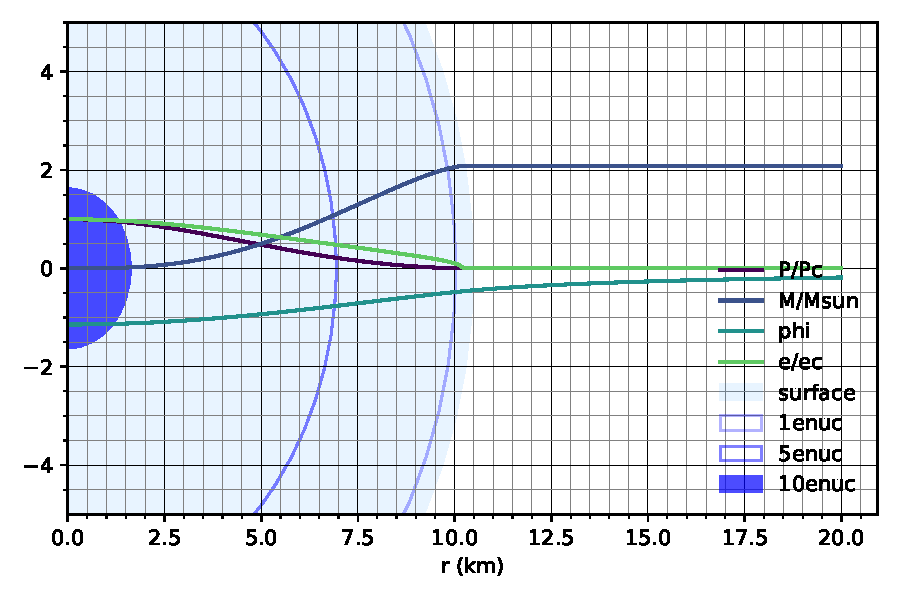
\includegraphics[width=0.5\textwidth]{utkarsh_images/ns_params_overplot.pdf}
\caption{\label{fig:2} NS Structure Overplot [Placeholder]}
\end{figure}
\begin{figure}[h]
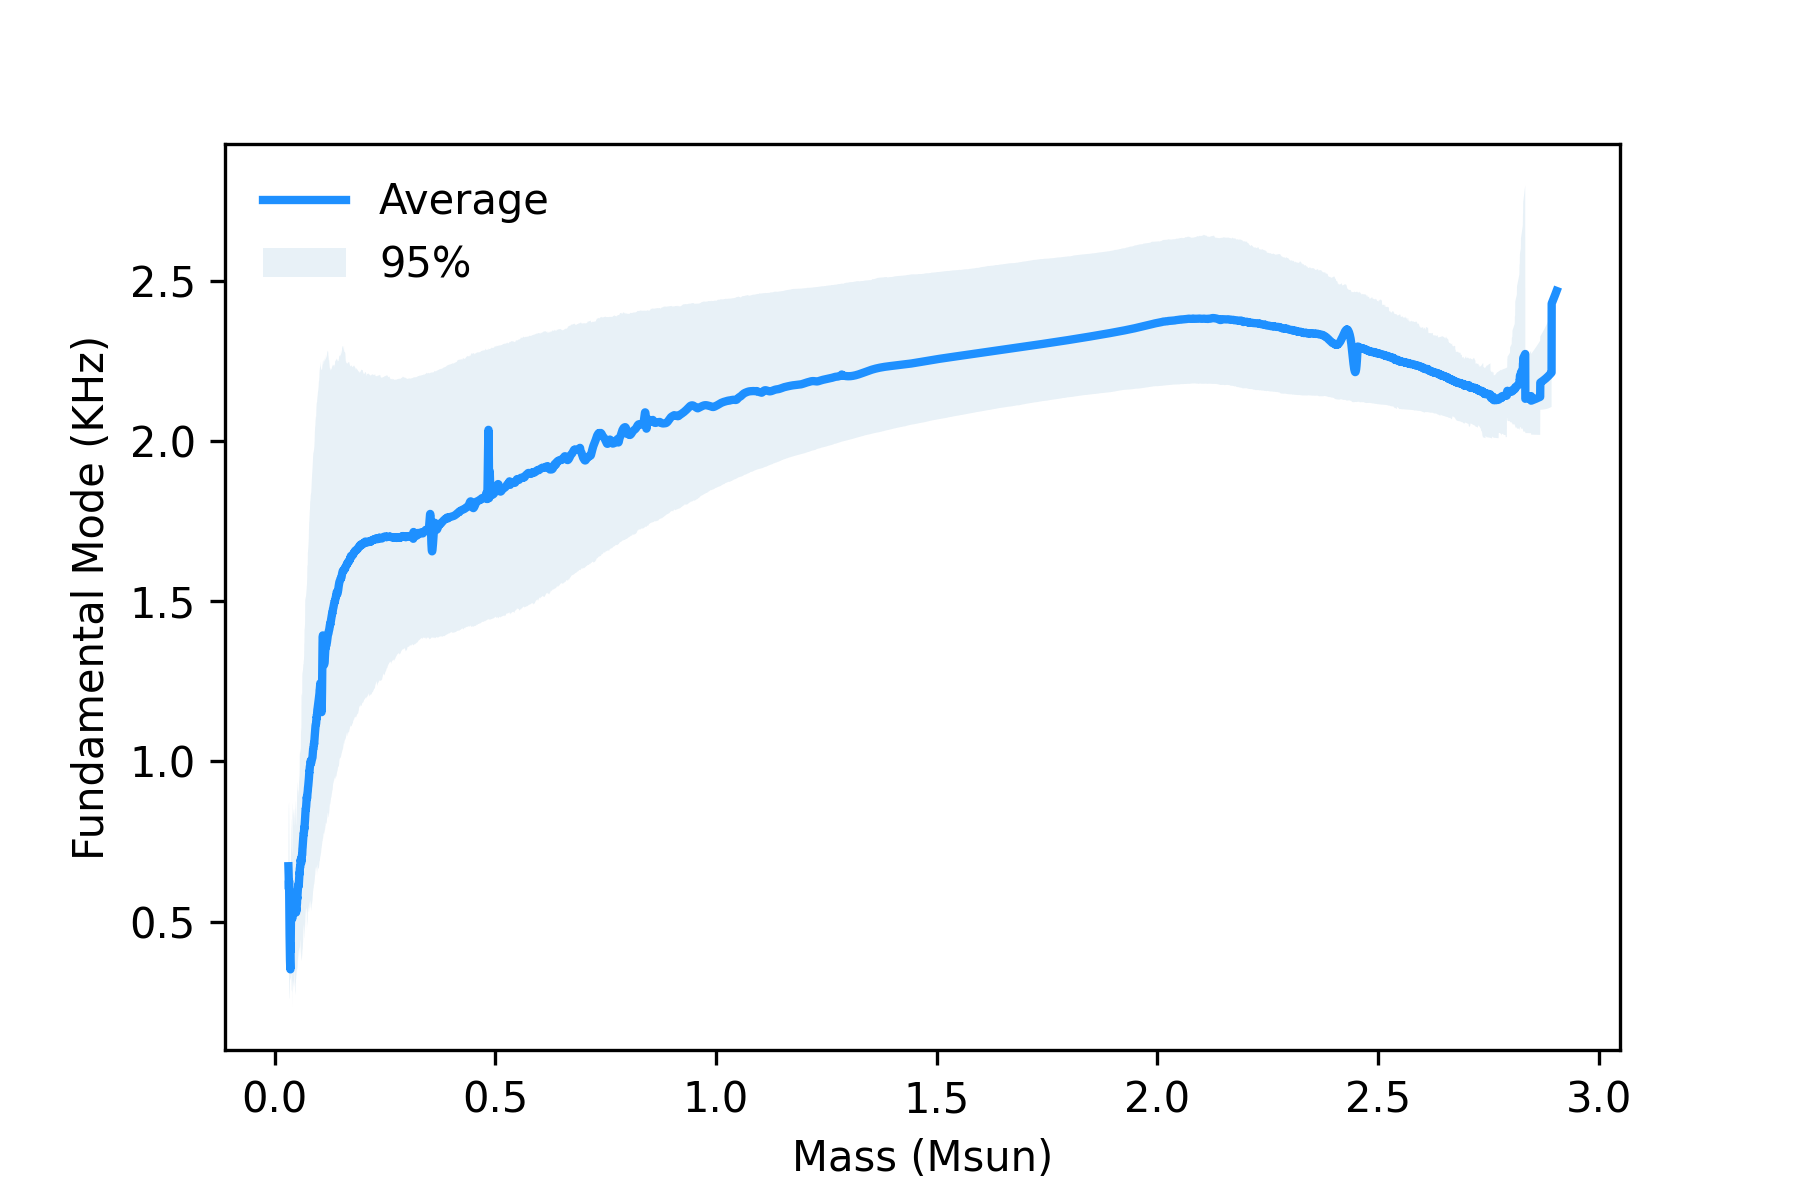
\includegraphics[width=0.5\textwidth]{utkarsh_images/fmode_envelope.png}
\caption{\label{fig:3} Envelope plot of fundamental modes in cowling approximation. 95\% confidence interval is shown. [Cowling Approximation]}
\end{figure}
\begin{figure}[h]
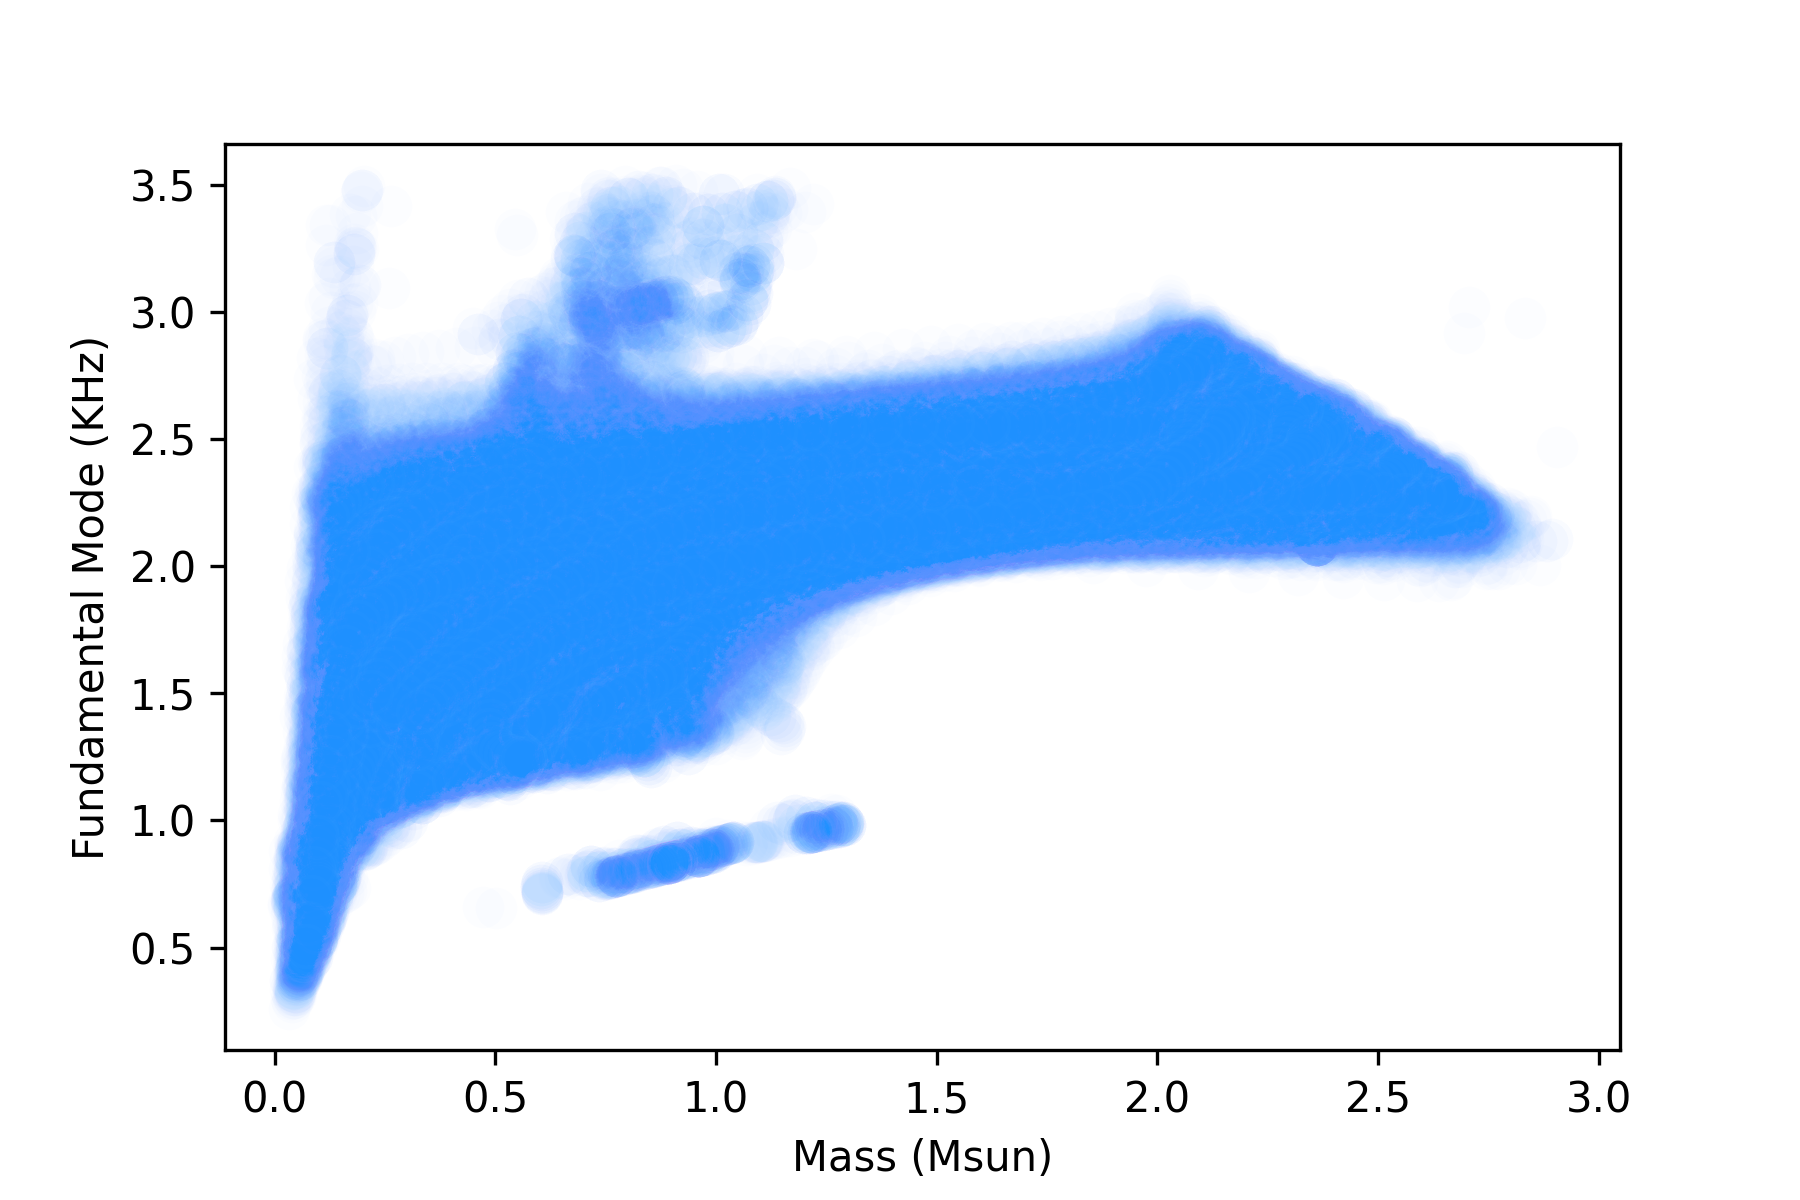
\includegraphics[width=0.5\textwidth]{utkarsh_images/fmode_scatter.png}
\caption{\label{fig:4} Scatter plot for fundamental modes vs mass relationship. Shaded region highlights high concentration of fmode vs mass relation. [Cowling Approximation]}
\end{figure}
\begin{figure}[h]
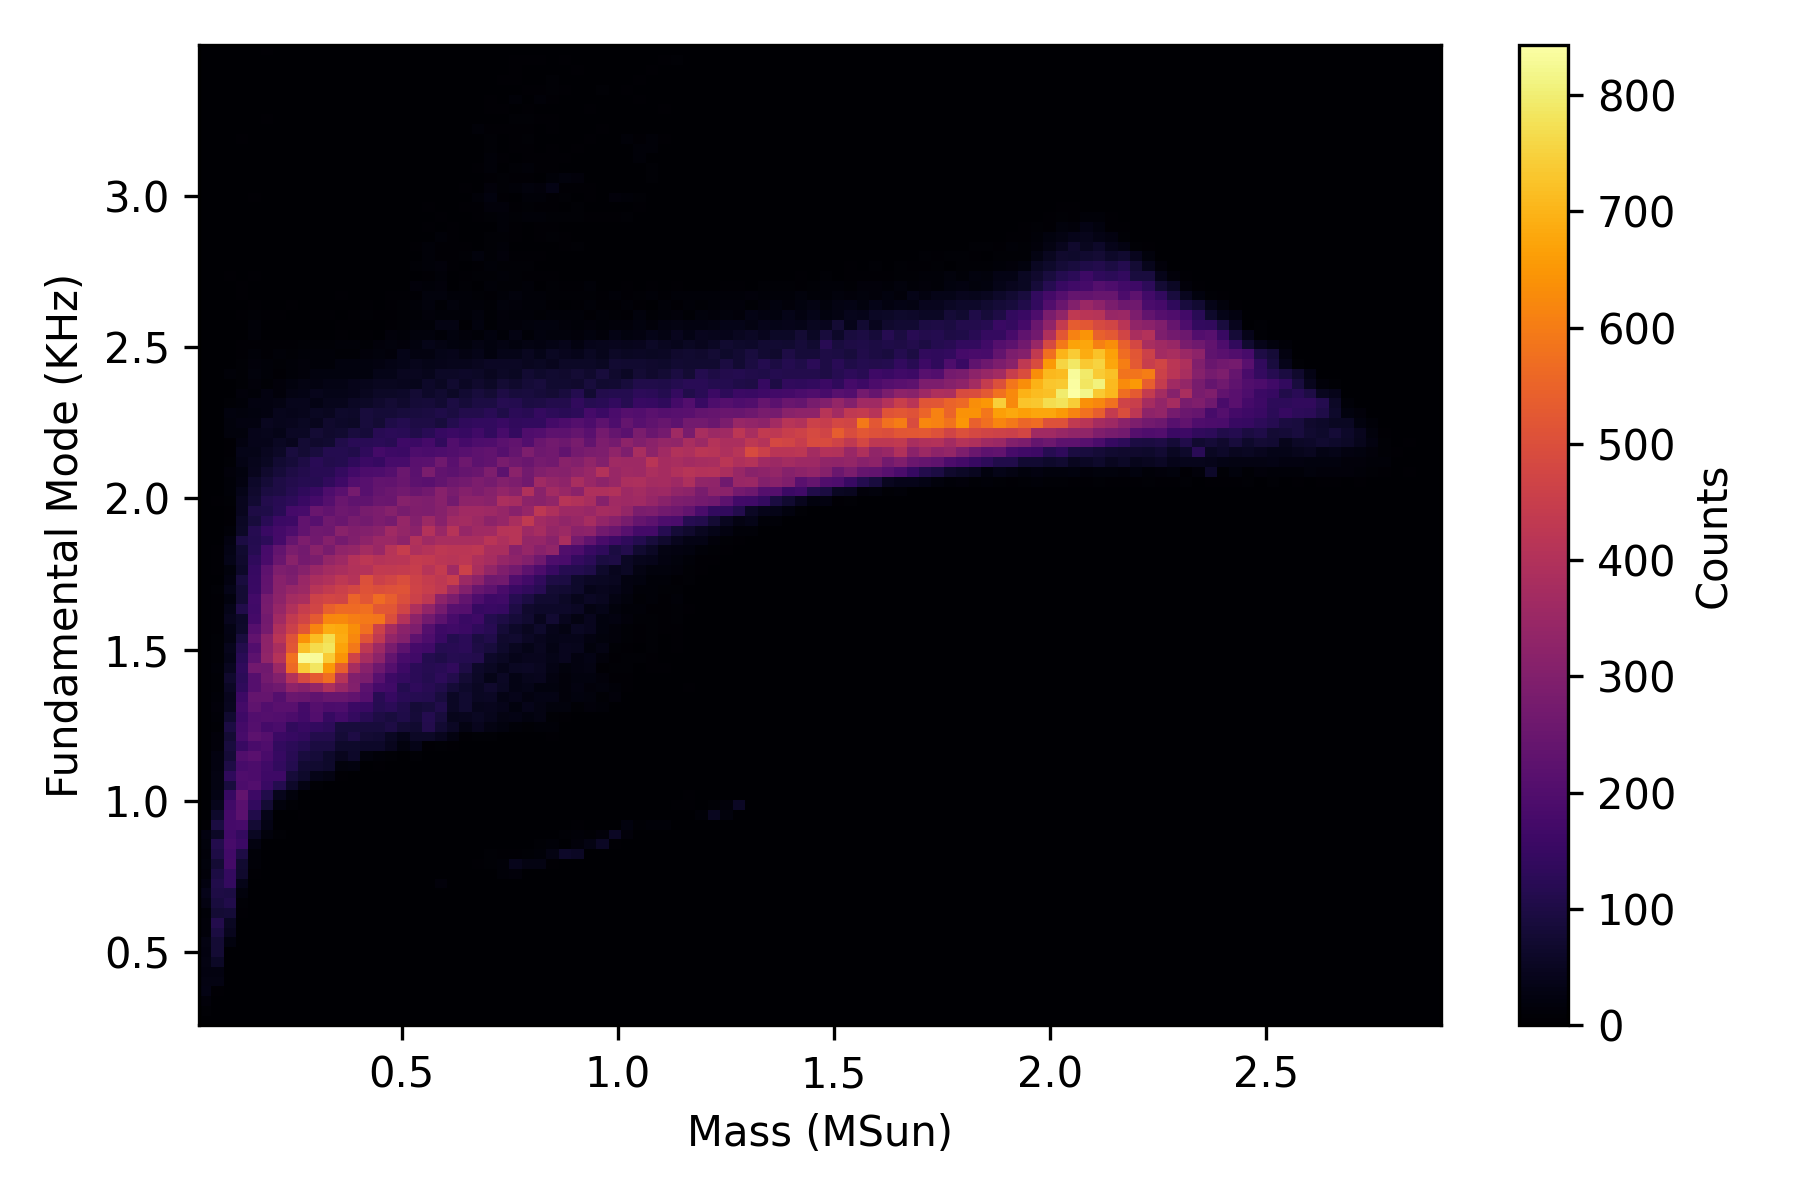
\includegraphics[width=0.5\textwidth]{utkarsh_images/fmode_bins.png}
\caption{\label{fig:5} Bins plot of fundamental mode vs mass of neutron star. Highlighted regions represent sharper concentration. [Cowling Approximation]}
\end{figure}
\begin{figure}[h]
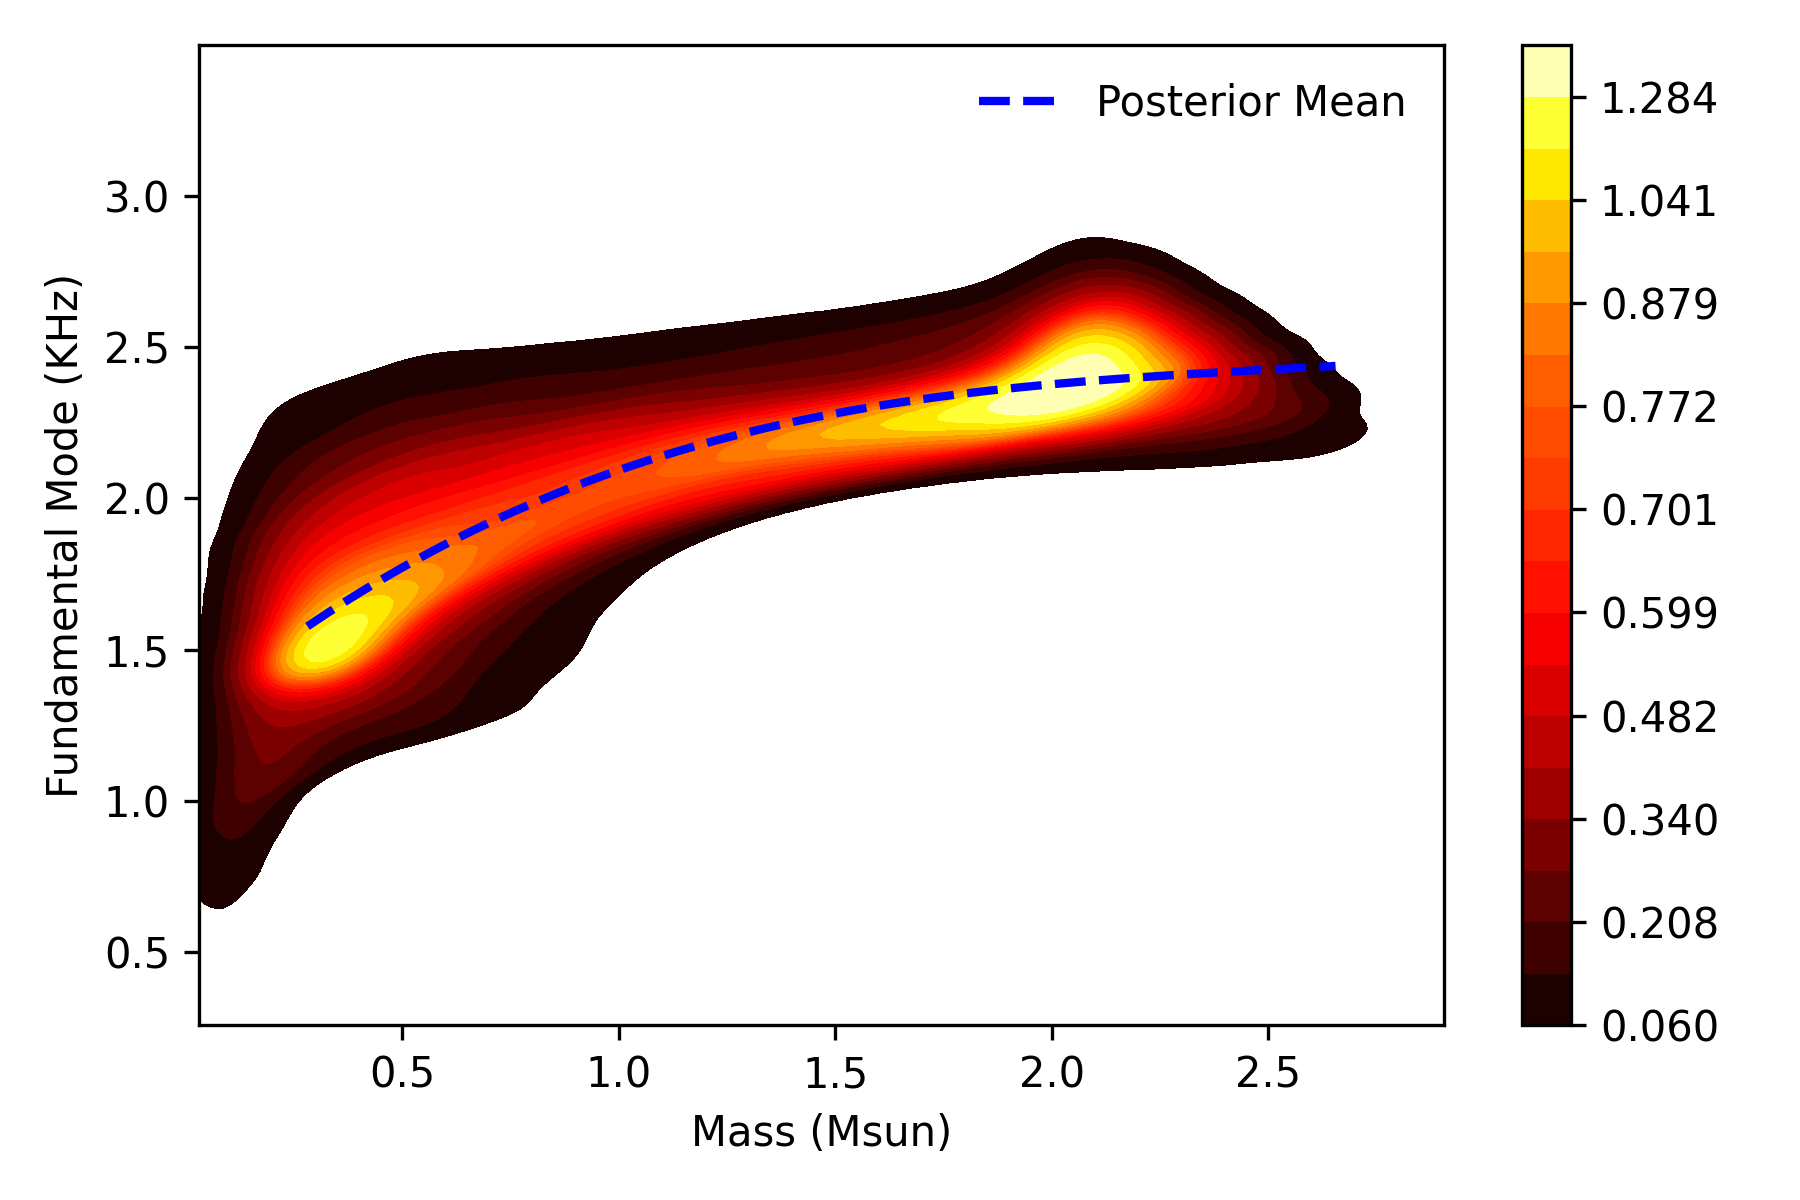
\includegraphics[width=0.5\textwidth]{utkarsh_images/fmode_contour.png}
\caption{\label{fig:6} Contour plot of fmode vs mass in the cowling approximation with the posterior mean over plotted. Lighted colours represent higher densities. [Cowling Approximation]} 
\end{figure}
\begin{figure}[h]
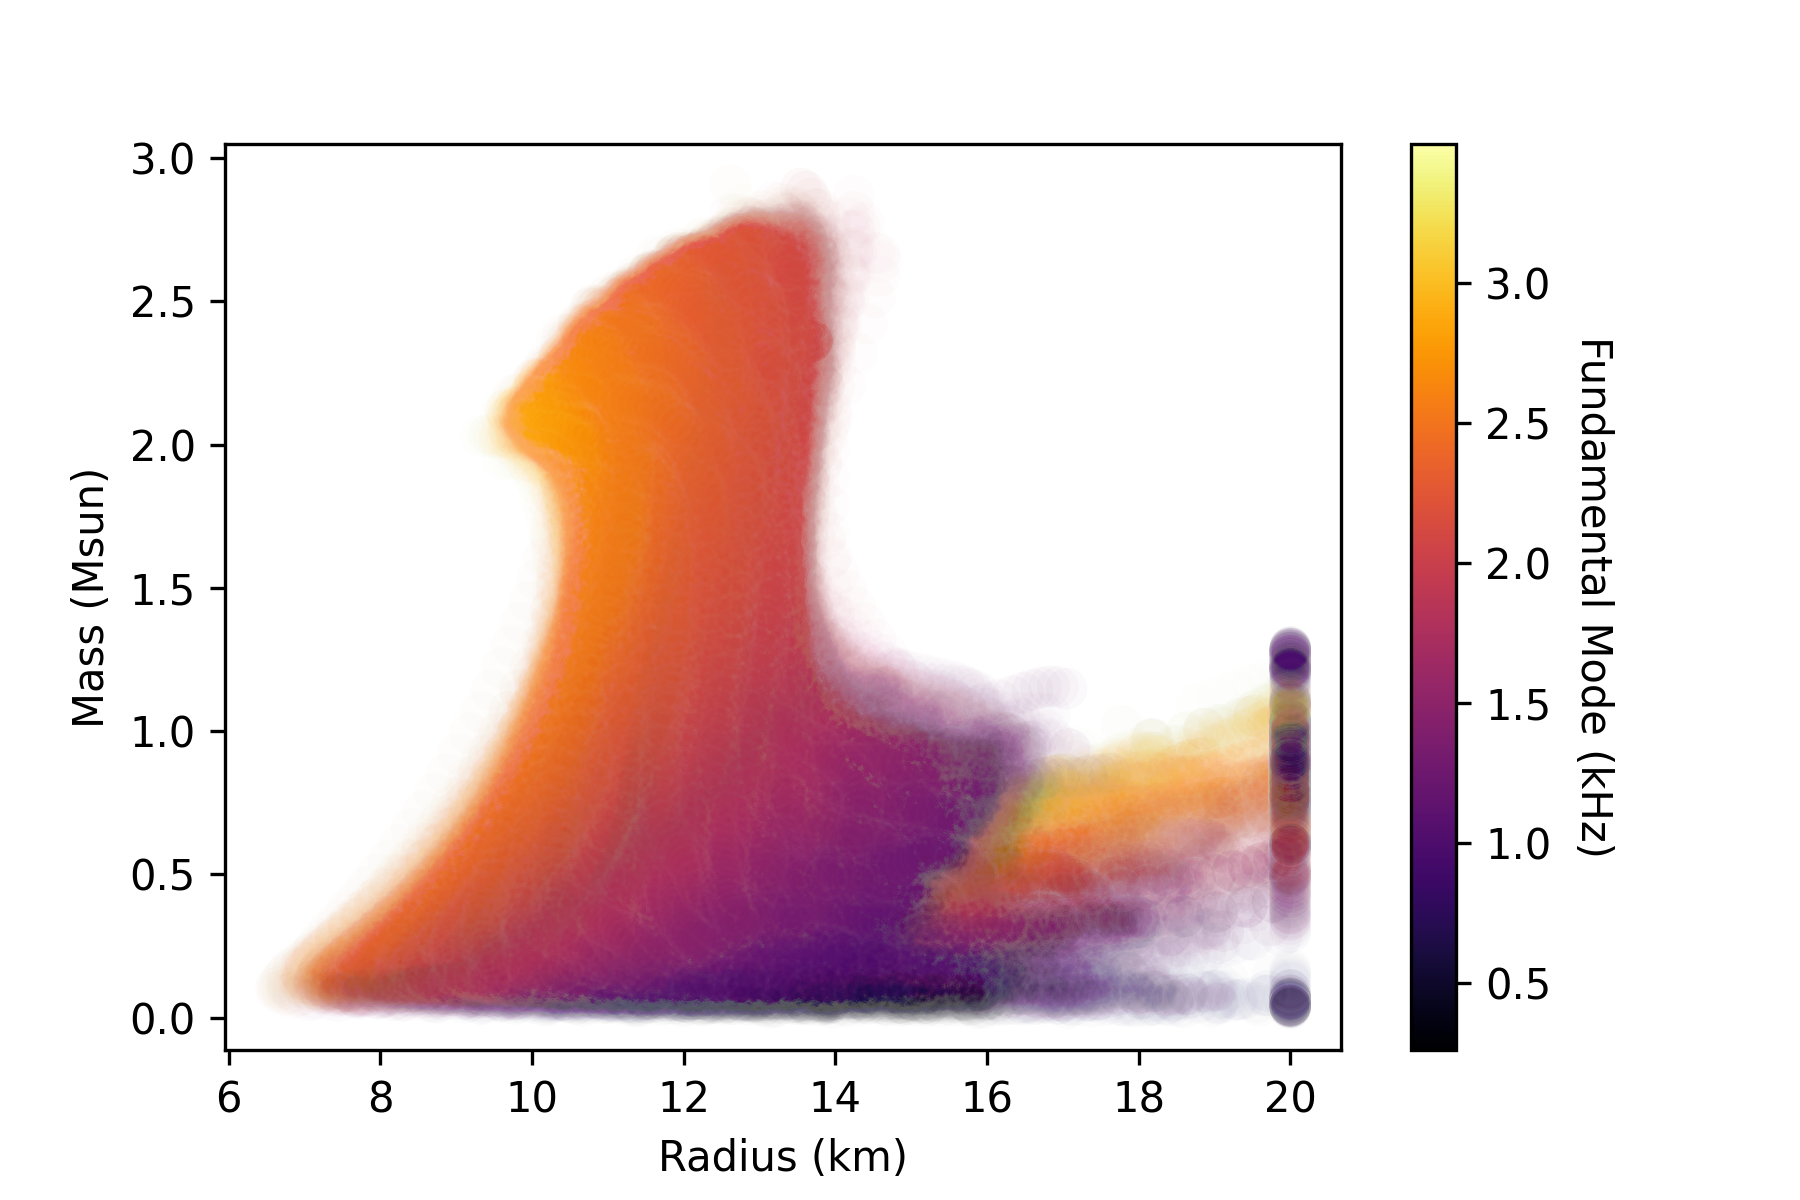
\includegraphics[width=0.5\textwidth]{utkarsh_images/fmode_MR.png}
\caption{\label{fig:7} Fundamental mode mass radius relationship with colour schematic of fundamental modes in the cowling approximation. Models drawn from EOS data. [Cowling Approximation]}
\end{figure}

Here, in Fig.~\ref{fig:fig1}, is an example figure.

\begin{figure}[!h]
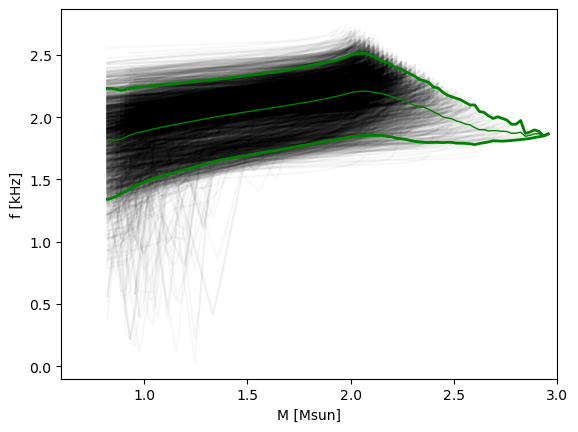
\includegraphics[width = \columnwidth]{fmode_psr+gw.png}
\caption{... \label{fig:fig1}}
\end{figure}

\section{Discussion}
Discuss and interpret the results, in the broader context of the research topic. State the main conclusions.

\acknowledgments
P.L. is supported by the Natural Sciences \& Engineering Research Council of Canada (NSERC).
%The authors are grateful for computational resources provided by the LIGO Lab and supported by NSF Grants PHY-0757058 and PHY-0823459.

\bibliographystyle{apsrev4-1}
\bibliography{references}

\end{document}